\clearpage
\section{Evaluation}

Zur Evaluierung wurde der Crawler auf einer einfachen rechteckigen Karte zufällig bewegt. Dabei wurde aus drei Bewegungsmöglichkeiten nach Tabelle \ref{tab:vars} probabilistisch eine ausgewählt, und ausgeführt, sofern dies ohne eine Kollision des Crawlers mit der Wand möglich ist. Die Position und Orientierung des Laufroboters werden parallel vom SE(2)-Filter und Partikelfilter geschätzt. Dann wird jeweils der Fehler zum Ground Truth berechnet. Für den Partikelfilter wurden 1000 eingesetzt, die Rotationskoordinate wurde in $mathtbb{S}$ berechnet.
In den Anfangsverteilungen wurden jeweils alle Koordinaten als stochastisch unabhängig voneinander angegeben.

\begin{table}[h!]
	\centering
	\caption{Mögliche Bewegungen}
	\label{tab:vars}
	\begin{tabular}{lll}
		\toprule
		Notation & Erklärung & Wahrscheinlichkeit\\
		\midrule
		$fwd$ 	& Schritt gerade nach vorne & 50\%\\
		$left$	& Drehung nach links		& 25\%\\
		$right$	& Drehung nach rechts		& 25\%\\

		\bottomrule
	\end{tabular}
\end{table}

Als Ground Truth wird der Crawler mit einer Deckenkamera getrackt. Über zwei verschiedenfarbige LEDs auf dem Crawler lässt sich dessen Position und Rotation bestimmen.

Aufgrund des hohen Zeitaufwands für das Aufnehmen von Bewegungspfaden des echten Crawlers, wurden zusätzlich in der Simulation erstellte zufällige Bewegungspfade als Ground Truth verwendet. Hierbei gibt es mehrere Möglichkeiten, welche Verteilung für das Rauschen im Systemmodell verwendet wird. Um den SE(2)-Filter nicht zu bevorteiligen, wenn im Systemmodell genau die Bingham-Verteilung des Filters verwendet wird, wurde eine weitere Testreihe mit Normalverteiltem Rauschen durchgeführt. Die hierfür benötigten Mittelwerte und Varianzen wurden für jeden der drei Freiheitsgrade $x,y,\theta$ unabhängig aus den Messdaten des Vorexperiments bestimmt.
Tabelle \ref{tab:testreihen} zeigt die insgesamt sechs Kombinationen aus den zwei Verfahren und drei Ground Truths. Für die Simulationen wurden die drei Karten aus Abbildung \ref{fig:map} mit jeweils 100 zufälligen Schritten betrachtet. Die Bewegungsbefehle waren für beide Verfahren pro Karte gemeinsam generiert. Für den realen Versuch wurde nur die quadratische Karte untersucht, mit zwei Bewegungsmustern von 60 und 40 zufälligen Schritten, die nacheinander ausgeführt wurden.
\begin{figure}
	\centering
	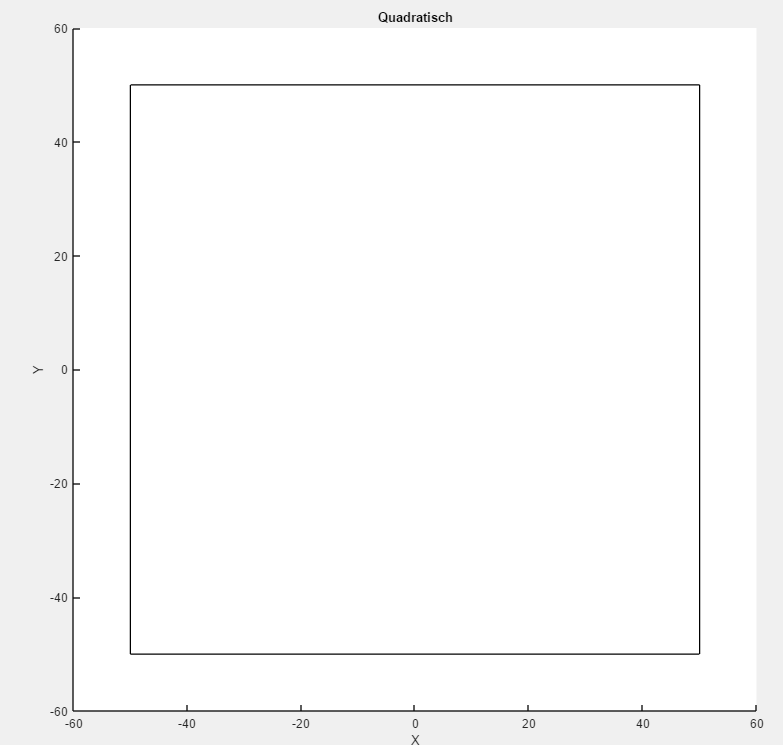
\includegraphics[width=0.32\linewidth]{Images/box.png}
	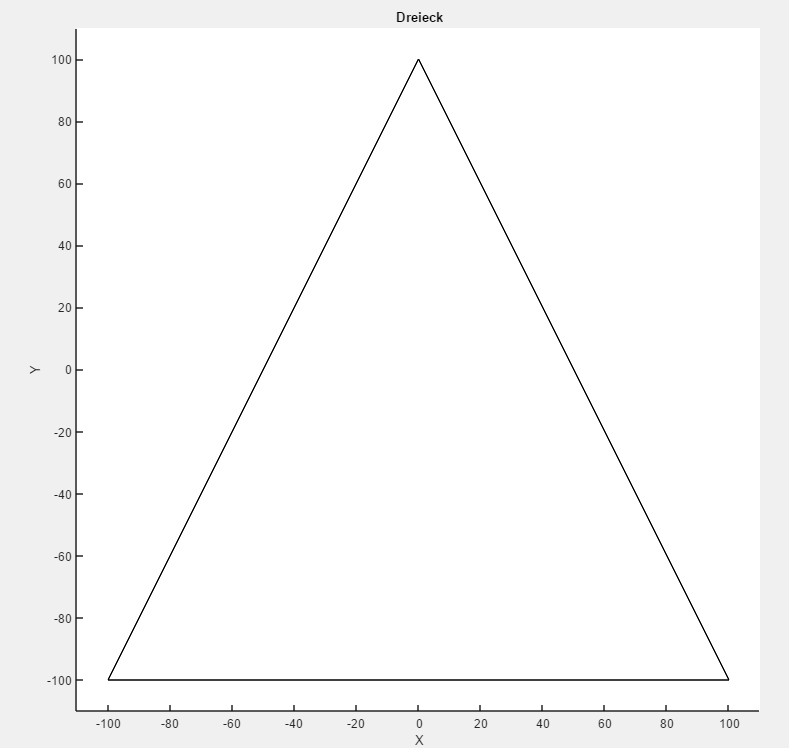
\includegraphics[width=0.32\linewidth]{Images/Dreieck.png}
	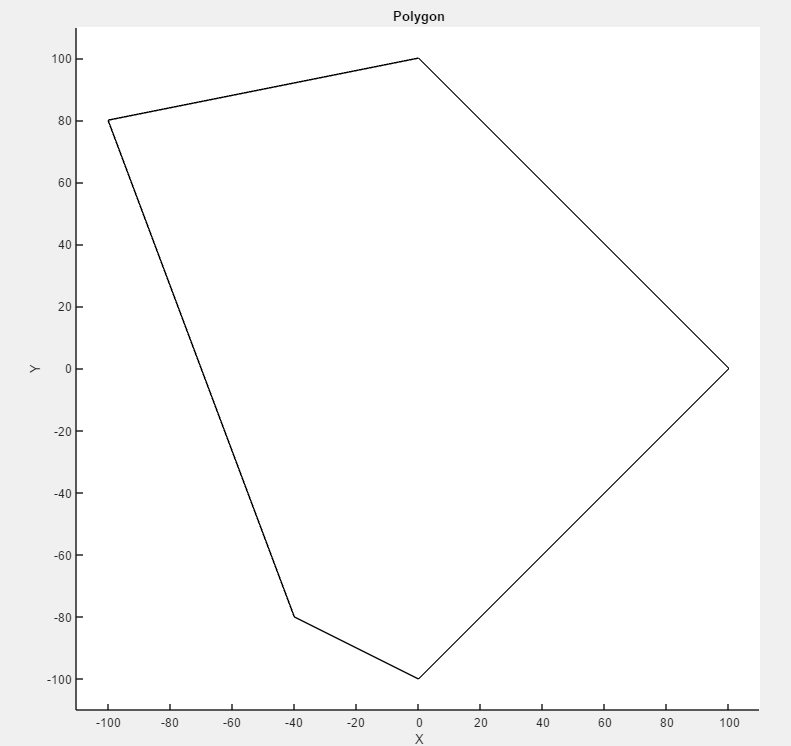
\includegraphics[width=0.32\linewidth]{Images/poly.png}
	\caption{Die drei zur Auswertung verwendeten Kartentypen}
	\label{fig:map}
\end{figure}

\begin{table}[h!]
	\centering
	\caption{Testreihen mit Anzahl Schritten}
	\label{tab:testreihen}
	\begin{tabular}{lll}
		\toprule
		Rauschen &  SE(2)-Filter &  Partikelfilter\\
		\midrule
		Normalverteilt 	& 300       & 300\\
		SE(2)-Bingham 	& 300		& 300\\
		Reale Daten 	& 60+40		& 60+40\\
		\bottomrule
	\end{tabular}
\end{table}


\subsection{Ergebnisse}

Tabelle \ref{tab:ergebnisse} stellt eine Übersicht der Evaluationsergebnisse. Die Fehlerdistanzen wurden über alle Schritte gemittelt.
Abbildung \ref{fig:gaussian} und \ref{fig:se2} zeigen den Fehlerverlauf von jeweils zwei Testreihen auf der quadratischen Karte. Hier wurde die euklidische Distanz zwischen der Position des Laufroboters und Ground Truth verwendet. Wie zu erwarten ist jeweils das Fiter-Verfahren, dessen angenommene Rauschverteilung mit der des tatsächlichen Systemmodells übereinstimmt etwas besser. Auffällig ist außerdem, dass beim SE(2)-Bingham-Rauschen der Fehler beider Verfahren deutlich größer ist.

Die Diagramme in Abbildung \ref{fig:roterror} zeigen den Rotationsfehler. Die unterschiedliche Zahl an Nulldurchgängen könnte ein Hinweis darauf sein, dass der Partikelfilter sich im Vergleich träger verhält.

Abbildung \ref{fig:real} zeigt den Positionsfehler für ein Bewegungsmuster des echten Crawlers. Die Lokalisations funktioniert deutliche schlechter, als in Simulation. Teilweise sogar gar nicht, wenn der Anfangszustand zur Initialisierung der Filter zu weit vom der tatsächlichen Position abweicht. Besonders empfindlich reagiert die Lokalisation, wenn der anfängliche Rotoationsfehler groß ist. Um einen signifikanten Unterschied zwischen den beiden Verfahren feststellen zu können, würde eine wesentlich größere Anzahl an aufgezeichneten Schritten des echten Crawler nötig werden.
Geringe Unterschiede in der Laufzeit lassen sich dennoch bemerkbar. Der Partikelfilter mit 100 Partikeln wertet die Messfunktion wesentlich häufiger aus, als der SE(2)-Filter mit dem Progressiven Update.

\begin{table}[h!]
	\centering
	\caption{Mittlere Fehler}
	\label{tab:ergebnisse}
	\begin{tabular}{lll}
		\toprule
		Rauschen &  SE(2)-Filter &  Partikelfilter\\
		\midrule
		Normalverteilt 	& 6.7       & 5.8\\
		SE(2)-Bingham 	& 7.5		&  8.8\\
		Reale Daten 	& 11.2		& 10.4\\
		\bottomrule
	\end{tabular}
\end{table}

\begin{figure}[h!]
	\centering
	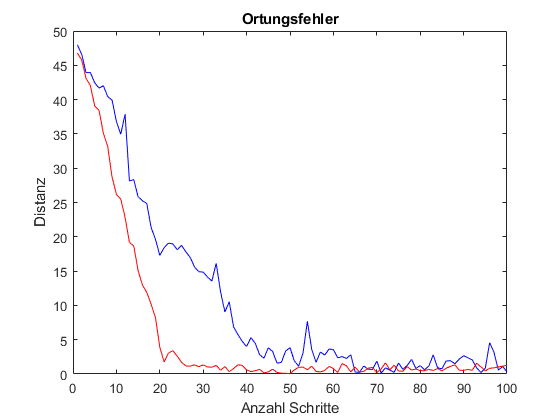
\includegraphics[width=0.7\linewidth]{Images/gaussianBox.png}
	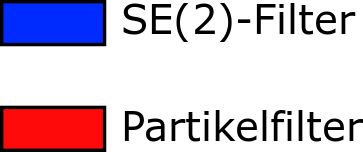
\includegraphics[width =0.1\linewidth]{Images/Legende.png}
	\caption{Normalverteiltes Rauschen}
    \label{fig:gaussian}
    
	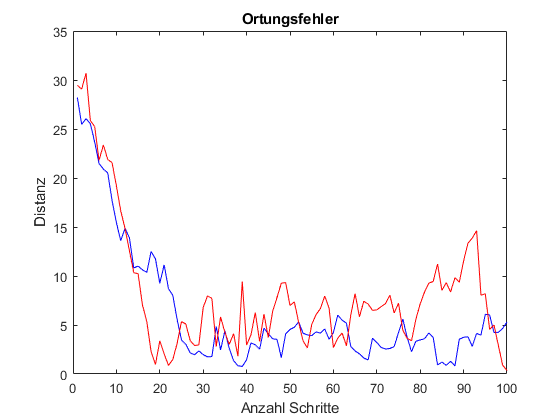
\includegraphics[width=0.7\linewidth]{Images/se2Box.png}
	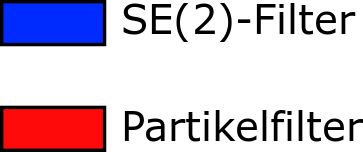
\includegraphics[width =0.1\linewidth]{Images/Legende.png}
	\caption{SE(2)-Bingham-verteiltes Rauschen}
	\label{fig:se2}
	\caption{Ergebnisse der Simulation mit Quadratischer Karte}
\end{figure}

\begin{figure}[h!]
	\centering
	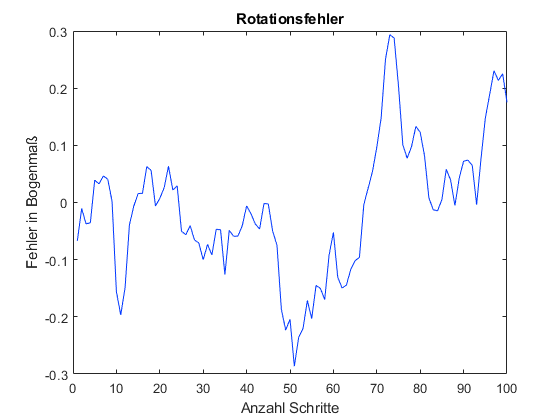
\includegraphics[width=0.40\linewidth]{Images/rotSE2.png}
	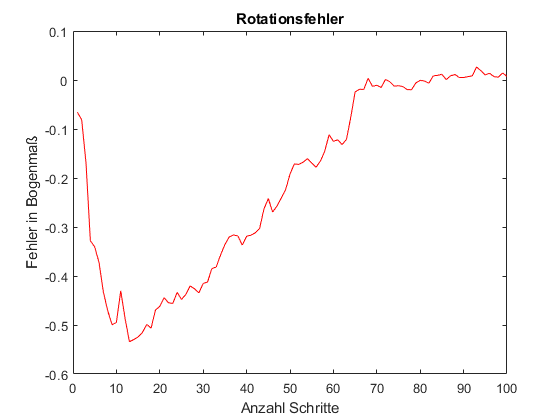
\includegraphics[width=0.40\linewidth]{Images/rotation.png}
	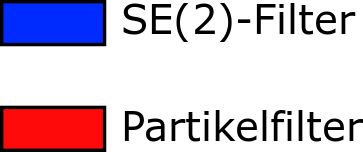
\includegraphics[width =0.18\linewidth]{Images/Legende.png}

	\caption{Rotationsfehler für quadratische Karte mit SE(2)-Bingham-Rauschen}
	\label{fig:roterror}
\end{figure}

\begin{figure}[h!]
	\centering
	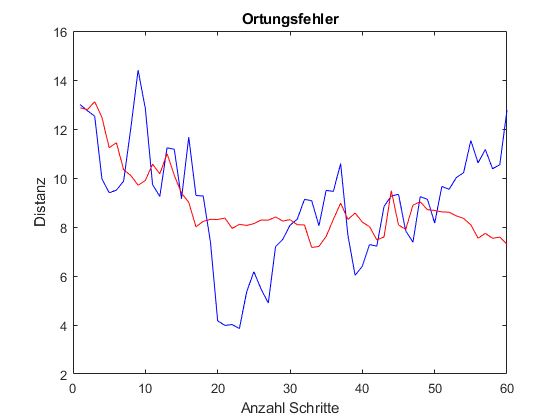
\includegraphics[width=0.60\linewidth]{Images/se2ErrorRealBoth.png}
	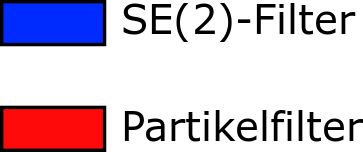
\includegraphics[width =0.18\linewidth]{Images/Legende.png}

	\caption{Fehler für die Bewegung des echten Crawlers}
	\label{fig:real}
\end{figure}
